\documentclass[11pt,oneside,parskip=half]{scrbook}
\usepackage[a4paper]{geometry}

\usepackage[dutch]{babel}
\usepackage[T1]{fontenc}
\usepackage[utf8]{inputenc}

\usepackage{amsmath}
\usepackage{amssymb}

\usepackage{pxfonts}

\usepackage{tabularx}
\usepackage{booktabs}
\usepackage{graphicx}

\usepackage{enumitem}

\usepackage{tikz}
\usetikzlibrary{calc}
\tikzstyle{every picture}=[thick]

\usepackage{listings}
\lstdefinelanguage{proto}
  {keywords={var, obj, clones, fun, returns, is,
             print, skip,
             if, then, else, while, do},
   emph={true, false, this, proto},
   %literate={==}{{$=$}}1 {/=}{{$\neq$}}1 {<=}{{$\leq$}}1 {>=}{{$\geq$}}1
   %         {+}{{$+$}}1 {-}{{$-$}}1 {*}{{$\times$}}1 {/}{{$/$}}
   %         {&}{{$\wedge$}}1 {|}{{$\vee$}}1 {~}{{$\lnot$}}1,
   comment=[l]{\#}}
\lstdefinelanguage{io}
  {keywords={clone, method, block, call, return,
             print, println,
             if, then, else, elsif,
             loop, repeat, while, for, break, continue},
   emph={true, false, nil, self, super},
   comment=[l]{\#}}
\lstdefinelanguage{class}[]{proto}
  {morekeywords={extends},
   deletekeywords={clones},
   moreemph={super},
   deleteemph={proto}}
\lstnewenvironment{program}{}{}
\lstMakeShortInline @
\lstset
  {language=proto,
   basicstyle=\small\ttfamily,
   emphstyle=\scshape,
   numbers=left,
   numberstyle=\small,
   numbersep=1em,
   mathescape=true,
   extendedchars=true}

\usepackage[nounderscore]{syntax}
\setlength{\grammarindent}{8em}
\renewcommand{\syntleft}{\normalfont\itshape}
\renewcommand{\syntright}{}

\newcommand\newkeyword[2]
  {\newcommand{#1}
     {\text{\scalebox{.95}{\small\ttfamily\bfseries #2}}}}
\newcommand\newconstant[2]
  {\newcommand{#1}
     {\text{\small\ttfamily\scshape #2}}}

\newcommand{\syn}[1]
  {\ensuremath{\mathit{#1}}}

\newcommand{\COMP}{;\;}
\newkeyword{\VAR}{local\;}
\newkeyword{\OBJ}{obj\;}
\newkeyword{\CLONES}{\;clones\;}
\newkeyword{\OBJECT}{\;object}
\newkeyword{\FUN}{function\;}
\newkeyword{\RETURNS}{\;returns\;}
\newkeyword{\IS}{\;is\;}
\newkeyword{\PRINT}{print\;}
\newkeyword{\SKIP}{skip}
\newkeyword{\IF}{if\;}
\newkeyword{\THEN}{\;then\;}
\newkeyword{\ELSE}{\;else\;}
\newkeyword{\WHILE}{while\;}
\newkeyword{\DO}{\;do\;}
\newkeyword{\END}{\;end}

\newconstant{\TRUE}{true}
\newconstant{\FALSE}{false}
\newconstant{\SELF}{self}
\newconstant{\PROTO}{proto}

\def\IN{\quad}

\def\I{\textit}

\newcommand{\<}
  {\ensuremath{\langle}}
\renewcommand{\>}
  {\ensuremath{\rangle}}

\frenchspacing% Cruciaal!
\raggedbottom% Handig

\newenvironment{SyntaxExample}{%
\vspace{-1.6pc}%
	\begin{equation*}%
		\begin{array}{l@{\hspace*{.02\textwidth}}|@{\hspace*{.02\textwidth}}l}%
		\hspace*{.35\textwidth} & \hspace*{.55\textwidth} \\[-1pc]%
}{%
		\end{array}%
	\end{equation*}%
\vspace{-.6pc}%
}

\def\DEF{\buildrel{\text{def}}\over{=}}
\def\Proto{\sqsubset^p}
\def\Outer{\sqsubset^s}
\def\ProtoEq{\sqsubseteq^p}
\def\OuterEq{\sqsubseteq^s}
\def\Attr{\mathit{attr}}
\def\SDef{\mathit{def}}
\newcommand{\ScopeID}[1]{\ensuremath{(1, #1)}}
\newcommand{\ObjectID}[1]{\ensuremath{(2, #1)}}

\begin{document}

\title{Een natuurlijke semantiek voor prototype oververing en lexicaal bereik}
\author{Kelley van Evert \& Tim Steenvoorden}
\maketitle

\frontmatter

\tableofcontents

\mainmatter

\chapter{Inleiding}

\begin{itemize}
	\item Motivatie
	\item JavaScript
	\item Lexical scope -- vrije/gebeonden variabelen
	\item Objecten en prototype overerving
\end{itemize}

\chapter{Notatie en terminologie}

\section{Beschouwing semantisch model}

We definieren in dit werkstuk een natuurlijke semantiek, d.w.z.~een ?-ste orde logica, met axioma's en deductieregels, en een bijbehorende structuur waarin deze zich afspeelt.

Deze structuur, die we ook wel het \emph{semantisch model} zullen noemen, heeft onderstaand opgesomde elementen. Deze worden verderop precies gedefinieerd, onderstaande opsomming geeft slechts een algemeen beeld.

\begin{description}
	\item[$\mathbb{M}$]\hfill\\ De verzameling mogelijke \emph{geheugens}, welke ook wel als \emph{eindtoestanden} worden geinterpreteerd.
	\item[$(\mathit{Stm} \times \mathbb{M} \times \mathbb{L} \times \mathbb{L})$]\hfill\\ De verzameling \emph{toestanden}, ook wel \emph{configuraties}.
	\item[$(\longrightarrow)$]\hfill\\ Een tweeplaatsig predikaat welke als eerste argument een element uit de verzameling van toestanden neemt, en als tweede argument een element uit de verzameling van eindtoestanden $(\mathbb{M}\dots)$. De uitspraak $(S, m, \sigma, \tau) \longrightarrow m'$ moet worden geinterpreteerd worden als:
	\begin{quote} ``Het programma $S$, met geheugen $m$, in scope $\sigma$ en met als $\mathbf{this}$ object $\tau$, resulteert in eindtoestand $m'$, mits $S$ \emph{correct} is''. \end{quote}
\end{description}

\section{Notationele conventies}

Terwille van elegantie houden we een aantal gebruikelijke notationele conventies aan:

\begin{enumerate}
	\item Voor elke twee willekeurige tweestemmige predikaten $\mathsf{S}$ en $\mathsf{T}$ (mogelijk ook $=$), en drie willekeurige elementen $a$, $b$ en $c$, definieren we de afkorting: $$a \operatorname{\mathsf{S}} b \operatorname{\mathsf{T}} c \buildrel{\mathrm{def}}\over{=} a \operatorname{\mathsf{S}} b \land b \operatorname{\mathsf{T}} c$$ in het geval dat deze bewering correct getypeerd is.
	\item Op eenzelfde manier definieren we ook de volgende afkorting: $$ \{a \in A \mid \phi \} \buildrel{\mathrm{def}}\over{=} \{a \mid a \in A \mid \phi\}$$
\end{enumerate}

[...]

\chapter{Taal en syntax}

In dit hoofdstuk zullen we de taal presenteren waarvoor we een natuurlijk taal construeren. De taal maakt gebruikt van prototype overerving en lexicaal bereik. Eerst zullen we een aantal voorbeeldprogramma's beschouwen, om zo informeel het karakter van de te formaliseren taal over te brengen. Daarna geven we een rigoreuze definitie met behulp van een BNF grammatica. De structuur van de productieregels van grammatica worden in latere hoofdstukken gebruikt om axioma's en deductieregels op te stellen. Daarmee heeft de grammatica in zekere zin een dubbele functie.

Elk voorbeeldprogramma en zijn toelichtingen worden als volg gepresenteerd:

	\begin{SyntaxExample}
		\VAR f & \textit{- variabelen moeten worden gedeclareerd} \\
		f = \FUN(i) \RETURNS n \\
		\IN \VAR n \\
		\IN n = 2 \times (i + 5) \\
		& \textit{- x bestaat niet in deze scope} \\
		\VAR x & \textit{- x is ongedefinieerd (maar wel aanwezig)} \\
		x = f(42) & \textit{- x = 89}
	\end{SyntaxExample}

De toelichtingen moeten als informeel commentaar worden beschouwd, waarmee we aan proberen te geven hoe het programma zich gedraagt. Vaak zijn het uitspraken over de toestand waarin het programma zich bevindt, direct na de linker regel te hebben ``uitgevoerd''.

\section{Voorbeeldprogramma's}

Een variabele moet gedeclareerd worden, en pas daarna kan er een waarde aan worden toegekend.

	\begin{SyntaxExample}
		& \textit{- x bestaat niet (in deze scope)} \\
		\VAR x & \textit{- x is ongedefinieerd (maar wel aanwezig)} \\
		x = 5 & \textit{- x = 5}
	\end{SyntaxExample}

Het concept van declaratie is juist in deze taal, gezien het lexicaal bereik van variabelen, heel belangrijk. Vergelijk het bovenstaande programma fragment bijvoorbeeld met de volgende situatie.

Variabelen hebben geen vaste type. Er zijn drie typen waarden in de taal: getallen, functies en objecten.

	\begin{SyntaxExample}
		\VAR x \\
		x = 5 & \textit{- de waarde van } x \textit{ is een getal} \\
		x = \FUN()\,\{\;\SKIP\;\} & \textit{- de waarde van x is een functie} \\
		x \OBJECT & \textit{- de waarde van x is een object}
	\end{SyntaxExample}

De taal is object georienteerd.

	\begin{SyntaxExample}
		\VAR o \\
		o \OBJECT \\
		& \textit{- o.f is niet gedefinieerd} \\
		o.f = \FUN()\,\{\;\SKIP\;\} & \textit{- toekenning waarde aan een attribuut van een object} \\
		& \textit{- o.f is wel gedefinieerd} \\
		o.n = 5 &
	\end{SyntaxExample}

Van de drie typen, zijn getallen en functies \emph{primitief}, en objecten \emph{niet primitief}. Primitieve waarde worden zelf gekopieerd (\emph{by-value}), maar van niet-primitieve waarden worden \emph{referenties} gekopieerd (\emph{by-reference}).

	\begin{SyntaxExample}
		\VAR x;\; x = 6 \\
		\VAR y;\; y = x & \textit{- x = 6 en y = 6} \\
		y = 7 & \textit{- x = 6 en y = 7} \\
		\\
		\VAR p;\; p.n = 6 \\
		\VAR q;\; q = p & \textit{- p en q verwijzen nu naar hetzelfde object} \\
		& \textit{- p.n = 6 en q.n = 6} \\
		q.n = 7 & \textit{- p.n = 7 en q.n = 7}
	\end{SyntaxExample}

\subsection{Lexicaal bereik / lexical scope}

Als in een zekere scope een variabele wordt gereferenceerd (nog) niet is gedefinieerd, wordt in omliggende scopes ``gezocht'' naar een definitie van deze variabele.

	\begin{SyntaxExample}
		\VAR x; \\
		\VAR f;\; f = \FUN(i) \\
		\IN x = i + 5 \\
		\\
		f(5) & \textit{- x = 10}
	\end{SyntaxExample}

..maar wanneer deze wel in de huidige scope bestaat, worden omliggende scopes ``met rust gelaten''.

	\begin{SyntaxExample}
		\VAR x \\
		\VAR f \\
		f = \FUN(i) \\
		\IN \VAR x \\
		\IN x = i + 5 \\
		\\
		f(5) & \textit{- x heeft nog geen waarde}
	\end{SyntaxExample}

Telkens wanneer een functie wordt aangeroepen, wordt een \emph{nieuwe scope} aangemaakt voor lokale variabelen. Variabelen van deze nieuwe scope kunnen later nog gereferenceerd worden, doordat bijvoorbeeld de functie een lokale functie teruggeeft.

	\begin{SyntaxExample}
		\VAR f \\
		f = \FUN(n) \RETURNS g \\
		\IN \VAR g \\
		\IN g = \FUN() \RETURNS n \\
		\IN \IN n = n + 1 \\
		\\
		\VAR c \\
		c = f(5) & \textit{- c() $\rightarrow$ 6, 7, 8, \dots}
	\end{SyntaxExample}

\fbox{maar dan wat beter geschreven, etc...}

\section{Grammatica}

[...en vervolgens helemaal formeel -- even uitleggen van BNF etc..]

\chapter{Semantisch model}

[Stukje bij beetje het semantisch model opbouwen, terwijl we steeds redeneren waarom we dat zo doen..]

\section{Scopes en lexical scope}

[Hierarchieen, outer scopes, bindingen, ``waarden'' kort noemen maar uitstellen tot ``Waarden: referenties en primitieven'']

\section{Objecten en prototype overerving}

[Graaf, bindingen, prototypen]

\section{Waarden: referenties en primitieven}

[Ze worden op dezelfde manier behandeld: objecten by-reference, dus de references zelf by-value, net als primitieven -- vandaar dat ze in dezelfde verzameling waarden zitten.]

\chapter{Natuurlijke Semantiek}

\chapter{Case study: Wiskundige formulering}

De vorm van bovenstaand semantisch model geeft een conceptueel sterk beeld van hoe de taal waarschijnlijk geimplementeerd zou worden in een compiler (modulo technische details, etc\dots). Het is ook vrijwel volgens bovenstaande semantiek dat aan informatica studenten object geörienteerde talen worden uitgelegd (referenties, primitieve waarden, \dots). Je kunt echter ook semantisch model maken wat ``wiskundiger van aard'' is. Daar zal dit hoofdstuk over gaan.

Belangrijke informatie, zoals welk object van welk ander object een prototype is en hoe de scopes elkaar bevatten, maar ook welke informatie binnen een object zit opgeslagen en welke variabelen in een scope zijn gedefiniëerd, worden ditmaal door relaties bevat.

Rest nog identificatie van objecten en scopes, deze zal op eenzelfde manier worden behandeld als eerder de ``locaties'' binnen het geheugen: ze moeten identiek zijn, maar verder is het van geen belang hoe ze worden gerepresenteerd. We zullen daarom aannemen dat er twee verzamelingen identifiers zijn, $\mathbb{S}$ en $\mathbb{O}$, waarbij bovendien:

\begin{enumerate}
	\item Voor beide verzamelingen $X \in \{\mathbb{S}, \mathbb{O}\}$, bestaat er een functie $\textsc{Next}:\mathcal{P}(X) \to X$, zdd $\textsc{Next}(Y) \notin Y$ voor alle $Y \subseteq X$.
	\item $\mathbb{S} \cap \mathbb{O} = \varnothing$ (Deze eis is niet een technische benodigdheid, maar geeft wel aan dat de semantiek van deze twee soorten identifiers nu eenmaal anders is.)
\end{enumerate}

De prototype hiërarchie, eveneens de scope hiërarchie, worden natuurlijk heel goed weergegeven door partiële ordeningen. Deze twee relaties zullen zullen we als $\Proto$ en $\Outer$, respectievelijk, noteren, en aannemen:

\begin{enumerate}
	\item $\Proto$ is een (tweestemmige) partiële ordening op $\mathbb{O}$
	\item $\Outer$ is een (tweestemmige) partiële ordening op $\mathbb{S}$
\end{enumerate}

Vervolgens introduceren we de relatie $\Attr \subseteq \mathbb{O} \times \mathit{Id} \times (\mathbb{O} \cup \mathbb{P})$. De uitspraak ``$p[i] = v$'' moet worden gelezen als: $(p, i, v) \in \Attr$. Deze relatie wordt eveneens gebruikt om de ``inhoud'' van objecten weer te geven, als de graafstructuur tussen objecten. Soortgelijk definiëren we de relatie $\SDef \subseteq \mathbb{S} \times \mathit{Id} \times (\mathbb{O} \cup \mathbb{P})$, waarbij de uitspraak ``$\sigma[i] = v$'' moet worden gelezen als: $(\sigma, i, v) \in \SDef$.

Ten alle tijde moeten de prototype en scope hiërarchieën, de inhoud van objecten en scopes, en de laatste indentificaties van objecten en scopes worden bijgehouden, en dit vormt dan het ``geheugen'', of de ``toestand'': $s = (\Attr, \SDef, \Proto, \Outer, p_\mathit{next}, \sigma_\mathit{next})$.

\begin{align*}
	\left<\SKIP, s, \tau, \sigma\right> &\longrightarrow s \\
	\left<x = e, s, \tau, \sigma\right> &\longrightarrow s[\; \sigma_d[x] = e \;] \\
	& \textbf{desda}\; \sigma_d = \max \{\, \sigma' \in \mathbb{S} \mid \sigma'[x] \land \sigma \OuterEq \sigma' \,\} \\
	\left<x \OBJECT, \tau, \sigma\right> &\longrightarrow s[\; \sigma_d[x] = p \;][\; p_\mathit{next} \mapsto p + 1 \;] \\
	& \textbf{desda}\; \sigma_d = \max \{\, \sigma' \in \mathbb{S} \mid \sigma'[x] \land \sigma \OuterEq \sigma' \,\} \\
	& \textbf{en}\; p = {p_\mathit{next}}_s
\end{align*}

\chapter{[...]}

%\chapter{Syntaxis}

\section{Grammatica}

Ik heb er een officiële \textsc{BNF}-grammatica van gemaakt en gezet met het @syntax@-pakket.
Enkele opmerkingen:
\begin{description}
  \item[Statements]
    \begin{itemize}
      \item Compositie gebeurt met een nieuwe regel,
        dit gegeven we aan met \Righttorque.
        Blokken geven we aan met behulp van inspringen,
        zodat we geen @end@ nodig hebben of haakjes.
      \item In plaats van @skip@ kunnen we dus ook \Righttorque gebruiken.
      \item @if@ en @while@ zijn standaard.
      \item @print@ om uitvoer van programma's te kunnen testen.
      \item @var@ is een \emph{declaratie}, en @=@ een \emph{toekenning}.
      \item @fun f() ...@ is een \emph{definitie}, @f()@ een \emph{aanroep}.
      \item Om objecten te kunnen klonen heb ik @obj A clones B@ verzonnen.
        Dit lijkt op het declareren van variabelen met @var@
        (maar dan @obj@ wegens objecten)
        en geeft een relatie tussen de objecten weer met @clones@.
        Dit kunnen we later eventueel uitbreiden naar klassen door
        @clones@ te vervangen door @extends@.
    \end{itemize}
  \item[Parameters \& Argumenten]
    Spreken redelijk voor zich. Achter de komma staat een spatie, aangegeven met \textvisiblespace.
  \item[Identifiers \& Slots]
    \begin{itemize}
      \item Onze ideeën over \emph{locaties} en \emph{paden}
        hernoemd naar \emph{slots}. Een slot is een plek waaronder
        je iets kunt opslaan (variabele, functie, object).
        Deze term wordt vaak gebruikt bij talen als Lua en IO.
      \item Identifiers bestaan gewoon uit kleine letters en hoofdletters.
        (Weet jij nog een goede manier om dit aan te geven zonder het hele
        alfabet op te noemen?)
      \item Het lijkt mij een goed idee om de namen van objecten te beginnen
        met een hoofdletter en variabelen en functies met een kleine.
    \end{itemize}
  \item[Expressies \& Operatoren]
    Alleen gehele getallen. Operatoren zijn standaard aritmetisch.
  \item[Tests \& Booleans]
    Speciale syntactische categorie zodat we ze alleen kunnen gebruiken binnen
    @if@ en @while@. Bevatten standaard logische operatoren.
    We kunnen de @&@ en @|@ ook vervangen door @&&@ en @||@ of @/\@ en @\/@,
    wat denk jij?
    Relaties zijn equivalentie en ordeningen op gehele getallen.
    Ik heb @true@ en @false@ woordelijk toegevoegd, overbodig of goed idee?
\end{description}

\begin{grammar}
<Statement>  ::= <Statement> \Righttorque <Statement>
            \alt \Righttorque
            \alt @if@ <Test> <Statement> @else@ <Statement>
            \alt @while@ <Test> <Statement>
            \alt @print@ <Expression>
            \alt @var@ <Slot> 
            \alt <Slot> "=" <Expression>
            \alt @fun@ <Slot> "(" <Parameters> ")" <Statement>
            \alt <Slot> "(" <Arguments> ")"
            \alt @obj@ <Slot> @clones@ <Slot>

<Parameters> ::= <Identifier> ",\ " <Parameters> | <Identifier>

<Arguments>  ::= <Expression> ",\ " <Arguments>  | <Expression>

<Slot>       ::= <Identifier> "." <Slot> | <Identifier>

<Identifier> ::= "a" | "b" | "c" | \dots

<Expression> ::= <Number>
            \alt <Slot>
            \alt <Expression> <Operator> <Expression>

<Operator>   ::= "+" | "-" | "*" | "/" | "\%"

<Number>     ::= "0" | "1" | "2" | "3" | \dots

<Test>       ::= <Boolean>
            \alt <Test> "\&" <Test>
            \alt <Test> "|"  <Test>
            \alt "~" <Test>
            \alt <Expression> <Relation> <Expression>

<Relation>   ::= "==" | "!=" | "<" | "<=" | ">" | ">="

<Boolean>    ::= @true@ | @false@
\end{grammar}

\section{Een programma over deuren}

Programma's kunnen we eenvoudig zetten met het @listings@-pakket. We kunnen @\begin{program}@ en @\end{program}@ gebruiken om programma's tussen te schrijven. Daarnaast heb ik het apenstaartje zo ingesteld dat alles tussen twee apenstaartjes in ``code''-modus worden gezet, inclusief het opmaken van sleutelwoorden!

\begin{program}
obj Door clones Object       // Maak een nieuwe deur

fun Door.open()              // Een functie om de deur te openen
    print 42

obj LockedDoor clones Door   // Maak een nieuwe gesloten deur...
var LockedDoor.isLocked
LockedDoor.isLocked = 1      // ...die dicht is

fun LockedDoor.unlock(code)
    if code == this.code     // Als de code correct is...
        isLocked = 0         // ...openen we de deur

fun LockedDoor.open()        // Herdefinieer om isLocked te gebruiken
    if isLocked == 1
        print 0
    else
        proto.open()         // Expliciete aanroep naar prototype

obj Safe clones LockedDoor   // Maak een kluis...
var Safe.code
Safe.code = 1234             // ...en ken een code toe

Safe.unlock(4321)
Safe.open()                  // Geeft 0, de deur is gesloten
Safe.unlock(1234)
Safe.open()                  // Geeft 42, we de juiste code hadden
\end{program}

\section{Een programma over personen}

\begin{program}
obj Person clones Object

var Person.total
Person.total = 0

fun Person.initialize()      // Wordt aangeroepen bij iedere kloon
    Person.total = Person.total + 1

obj Me clones Person
var Me.age
Me.age = 37

obj You clones Person
var You.age
You.age = 42

print Person.total           // Geeft 2
\end{program}

\section{Een programma over scope}

\begin{program}
var x
x = 1
fun g()
    print x
    x = 2
fun f()
    var x
    x = 3
    g()
f()
print x
\end{program}

% vim: spell spl=nl

%\chapter{Vergelijking met IO}

\section{Grammatica}

\begin{grammar}
<Statement>  ::= <Statement> ";" <Statement>
            \alt "nil"
            \alt "if" "(" <Test> "," <Statement> "," <Statement> ")"
            \alt "while" "(" <Test> "," <Statement> ")"
            \alt <Expression> "println"
            \alt <Slot> ":=" <Expression>
            \alt <Slot>  "=" <Expression>
            \alt <Slot> ":=" "method" "(" \{ <Identifier> "," \} <Statement> ")"
            \alt <Slot> ":=" <Slot> "(" [ <Expression> \{ "," <Expression> \} ] ")"
            \alt <Slot> ":=" <Slot> "clone"

<Slot>       ::= <Identifier> \{ "\ " <Identifier> \}

<Identifier> ::= ( "a" | \dots | "z" | "A" | \dots | "Z" | "_" )+

<Expression> ::= <Number>
            \alt <Slot>
            \alt <Expression> <Operator> <Expression>

<Operator>   ::= "+" | "-" | "*" | "/"

<Number>     ::= ( "0" | \dots | "9" )+

<Test>       ::= <Boolean>
            \alt <Test> "and" "(" <Test> ")"
            \alt <Test> "or" "(" <Test> ")"
            \alt "not" "(" <Test> ")"
            \alt <Expression> <Relation> <Expression>

<Relation>   ::= "==" | "!=" | "<" | "<=" | ">" | ">="

<Boolean>    ::= "true" | "false"
\end{grammar}

\newpage
\section{Doors}

\begin{minipage}{0.5\textwidth}
\begin{program}
obj Door clones Object

fun Door.open() is
    print 42

obj LockedDoor clones Door
var LockedDoor.isLocked
LockedDoor.isLocked = 1

fun LockedDoor.unlock(code) is
    if code == this.code then
        isLocked = 0

fun LockedDoor.open() is
    if isLocked == 1 then
        print 0
    else
        proto.open()

obj Safe clones LockedDoor
var Safe.code
Safe.code = 1234

Safe.unlock(4321)
Safe.open()
Safe.unlock(1234)
Safe.open()
\end{program}
\end{minipage}
\begin{minipage}{0.5\textwidth}
\lstinputlisting[language=io]{doors.io}
\end{minipage}

\newpage
\section{Persons}

\begin{minipage}{0.5\textwidth}
\begin{program}
obj Person clones Object

var Person.total
Person.total = 0

fun Person.initialize() is
    Person.total = Person.total + 1

obj Me clones Person
var Me.age
Me.age = 37

obj You clones Person
var You.age
You.age = 42

print Person.total
\end{program}
\end{minipage}
\begin{minipage}{0.5\textwidth}
\lstinputlisting[language=io]{persons.io}
\end{minipage}

\section{Scope}

\begin{minipage}{0.5\textwidth}
\begin{program}
var x
x = 1
fun g() is
    print x
    x = 2
fun f() is
    var x # Weghalen geeft dynamic
    x = 3
    g()
f()
print x
\end{program}
\end{minipage}
\begin{minipage}{0.5\textwidth}
\lstinputlisting[language=io]{scope.io}
\end{minipage}

\newpage
\section{Counters}

\begin{minipage}{0.5\textwidth}
\begin{program}
fun counter(n) returns next is
    fun next() returns n is
        n = n + 1

var c
c = counter(5)

var d
d = counter(42)

var i, j
i = c()
j = d()
\end{program}
\end{minipage}
\begin{minipage}{0.5\textwidth}
\begin{lstlisting}[language=io]
counter := block(n,
    block(
        n = n + 1))


c := counter call(5)


d := counter call(42)


i := c call
j := d call
\end{lstlisting}
\end{minipage}

\begin{minipage}{0.5\textwidth}
\begin{program}
obj Counter clones Object
var Counter.n
fun Counter.next() is
    n = n + 1

obj c clones Counter
c.n = 5

obj d clones Counter
d.n = 42


c.next()
d.next()
\end{program}
\end{minipage}
\begin{minipage}{0.5\textwidth}
\begin{lstlisting}[language=io]
Counter := Object clone

Counter next := method(
    n = n + 1)

c := Counter clone

c n := 5

d := Counter clone

d n := 42

c next
d next
\end{lstlisting}
\end{minipage}

% vim: ft=context

%\chapter{Troep}

\section{Regels}

\subsection{While}

@$\<$while not (x = 1) do y = y * x; x = x - 1$, s_{3,2}\> \to s_{6,1}$@

$\<\WHILE x \neq 1 \DO y = y \times x;~ x = x - 1, s_{3,2}\> \to s_{6,1}$

$\<\mathtt{while}(x \neq 1, y = y \times x;~ x = x - 1), s_{3,2}\> \to s_{6,1}$

$\<\FUN counter(n) \RETURNS next \IS (\FUN next() \RETURNS n \IS n = n + 1), s\>$

$\<\FUN counter(n) \RETURNS next \IS \FUN next() \RETURNS n \IS n = n + 1 \END \END, s\>$

$\<counter := \mathtt{block}(n, \mathtt{block}(n = n + 1)), s\>$

$\<\VAR x\COMP x=1\COMP
   \FUN g() \IS (\PRINT x\COMP x=2)\COMP
   \FUN f() \IS (\VAR x\COMP x=3\COMP g())\COMP
   f()\COMP
   \PRINT x,
s\> \to s'$


$\<\VAR x\COMP x=1\COMP
   \FUN g() \IS \PRINT x\COMP x=2 \END\COMP
   \FUN f() \IS \VAR x\COMP x=3\COMP g() \END\COMP
   f()\COMP
   \PRINT x,
s\> \to s'$

$\<x:=1;~
   g:=\mathtt{method}(x \mathtt{~print};~ x=2);~
   f:=\mathtt{method}(x:=3;~ g());~
   f();~
   x \mathtt{~print}, 
s\> \to s'$

$\<x:=1;
   g:=\mathtt{block}(x \mathtt{~println}; x=2);
   f:=\mathtt{block}(x:=3; g \mathtt{~call});
   f \mathtt{~call};
   x \mathtt{~println}, 
s\> \to s'$

\subsection{Fun}

\<@fun $f$($y$) {$x$ = $y$}@, $s$, $\epsilon$\> $\to (s',\epsilon)$

@$\<$fun $f$($y$) {$x$ = $y$}$, s, \epsilon\> \to (s',\epsilon)$@

\<@fun f(y) {x = y}@, $s$, $\epsilon$\> $\to (s',\epsilon)$

$\<\FUN f(y) \IS x = y, s, \epsilon\> \to (s', \epsilon)$

---

$\< \mathbf{fun}\;f(y)\;\;\{x=y\}, s, \epsilon \> \to s'$

$\<\texttt{\FUN\ f(y) \{x = y\}}, s, \epsilon\> \to s'$

$\<\syn{fun f(y) {x = y}}, s, \epsilon\> \to s'$

%$\<@fun@ f@(@y@)@ @{@ x @=@ y@}@, s, \epsilon\> \to s'$

$\<\mathtt{fun} f(y) \{x = y\}, s, \epsilon\> \to s'$

\<@fun@ $f$@(@$y$@)@ @{@ $x$@=@$y$ @}@, $s$, $\epsilon$\> $\to s'$

--- ---

\subsection{If}

\<@if $T$ $S_1$ else $S_2$@, $s$, $\epsilon$\> $\to (s',\epsilon)$

@$\<$if $T$ $S_1$ else $S_2, s, \epsilon\> \to (s',\epsilon)$@

\<@if b T else F@, $s$, $\epsilon$\> $\to (s',\epsilon)$

---

$\<\syn{if T S1 else S2}, s\> \to s'$

$\<\IF\; T\; S_1\; \ELSE\; S_2, s\> \to s'$

%$\langle @if@ T S_1 @else@ S_2, s \rangle \to s'$

$\langle$@if T S1 else S2@$\rangle$

@$\langle$ if $T$ $S_1$ else $S_2$ $\rangle$@

\<@if@ $T$ $S_1$ @else@ $S_2$, $s$\> $\to s'$

%$\< @if@\; T\; S_1\; @else@\; S_2, s \> \to s'$

$\< \IF T S_1 \ELSE S_2 \> \to s'$

%\tuple{@if@ $T$ $S_1$ @else@ $S_2$}$\to s'$

\section{Bomen}

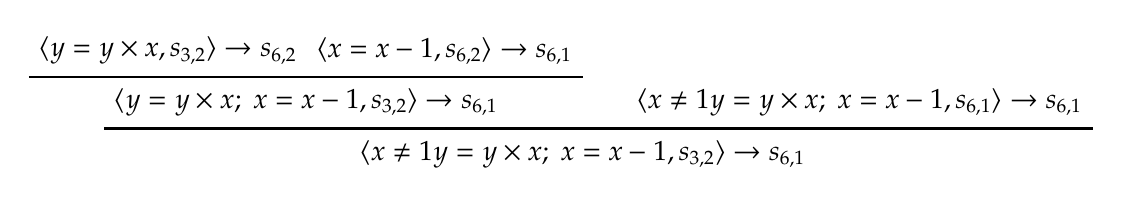
\begin{tikzpicture}
   [edge from parent path={
      ($(\tikzchildnode.west) - (0,0.5\tikzleveldistance)$)
      -- ($(\tikzchildnode.east) - (0,0.5\tikzleveldistance)$)
      ($(\tikzparentnode.west) + (0,0.5\tikzleveldistance)$)
      -- ($(\tikzparentnode.east) + (0,0.5\tikzleveldistance)$)
    },
    grow'=up,
    level/.style={sibling distance=20em/#1},
    level distance=4ex]
    \node {$\<\WHILE x \neq 1 \DO y = y \times x\COMP x = x - 1, s_{3,2}\> \to s_{6,1}$}
    child { node {$\<y = y \times x\COMP x = x - 1, s_{3,2}\> \to s_{6,1}$}
      child { node {$\<y = y \times x, s_{3,2}\> \to s_{6,2}$} }
    child { node {$\<x = x - 1, s_{6,2}\> \to s_{6,1}$} } }
  child { node {$\<\WHILE x \neq 1 \DO y = y \times x\COMP x = x - 1, s_{6,1}\> \to s_{6,1}$} };
\end{tikzpicture}

% vim: ft=context


\backmatter

\end{document}

% vim: ft=context
